\clearpage
\subsection{Can a consistency check rescue a one-choice screen?}
The $\mathrm{CaZrO_3}$ failure suggests a testable diagnostic. Define
\[
 D(z)=\big|\hat g(z)-(\hat v(z)-\hat c(z))\big|.
\]
All three terms are predictions from the property-first model, so the diagnostic could be computed before measuring a candidate. It checks whether the two representations of the gap agree. A small residual can also occur when both representations are wrong in the same direction.

\begin{figure}[ht]
\centering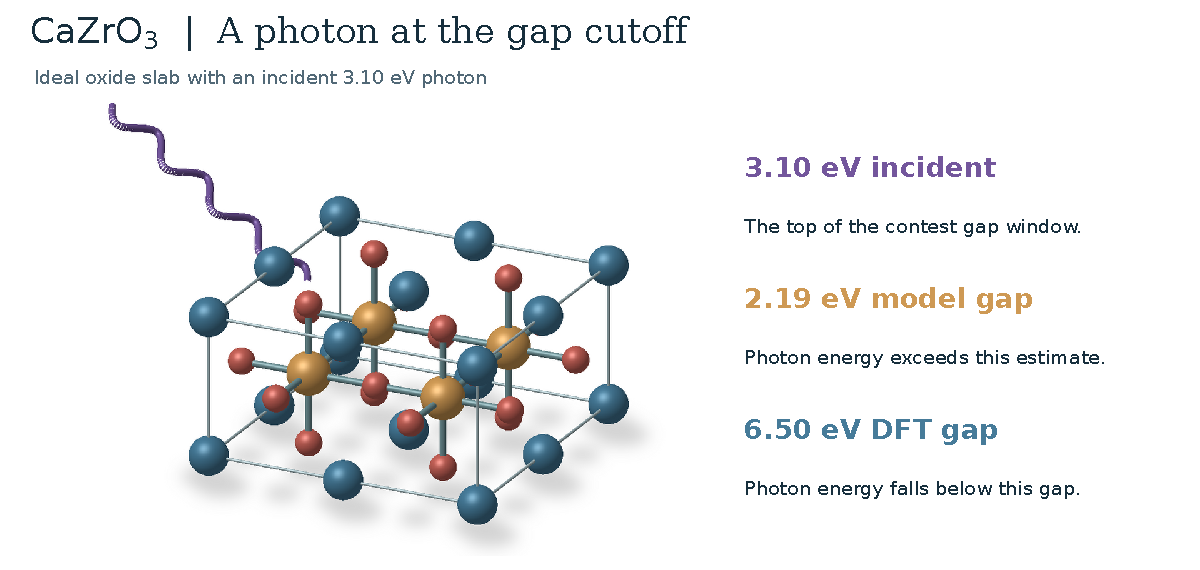
\includegraphics[width=.95\linewidth]{figures/property_tests.pdf}
\caption{An incident photon at the 3.10 eV screening cutoff approaches an ideal fragment of $\mathrm{CaZrO_3}$. The wave is symbolic. Its energy exceeds the model gap but falls below the public DFT gap. This compares energy thresholds only; the files supply no absorption spectrum for this illustration.}\label{fig:physicaltests}
\end{figure}

At 3.10 eV, a photon carries about the energy of 400 nm light ($\lambda=hc/E$). Figure~\ref{fig:physicaltests} uses it to expose the practical consequence of the gap discrepancy. Whether a transition actually absorbs light also depends on selection rules and the optical response.

We test a veto on the 1,701 Q3 validation records: discard predictions with $D>\tau$ and select the remaining candidate with the smallest property-first violation. Table~\ref{tab:veto} reports both seeds, with 26 first in each entry. The same 11 near-targets are available to each fit. Thresholds are exploratory, and this test does not alter the frozen mixture.
\begin{table}[ht]
\caption{Cost of vetoing inconsistent property predictions. Eligible and retained counts refer to distinct Q3 validation records.}\label{tab:veto}
\centering\small\begin{tabular}{lrrr}
\toprule Tolerance (eV) & Eligible records & Near-targets retained & First observed $V$\\\midrule
No veto & 1701 / 1701 & 11 / 11 & 46.24 / 46.24\\
1.00 & 1698 / 1699 & 11 / 10 & 11.25 / 46.24\\
0.50 & 1690 / 1681 & 10 / 9 & 11.97 / 11.25\\
0.25 & 1634 / 1623 & 7 / 5 & 11.97 / 10.88\\
0.05 & 753 / 805 & 0 / 3 & 10.88 / 10.93\\\bottomrule
\end{tabular}
\end{table}

At $\tau=0.50$ the large error on $\mathrm{CaZrO_3}$ is removed for both seeds, yet neither replacement is a near-target. At $\tau=0.05$ the seed-26 screen eliminates every available near-target. Agreement between model outputs can flag a case for inspection. Using that agreement as an automatic rejection criterion sacrifices some of the materials the screen is meant to find.

